%! TEX root = **/010-main.tex
% vim: spell spelllang=en:

\section{Description of pre-processing of data}%
\label{sec:desc-prep}

% Kind of preprocessing done to the original data:  Have you simplified the dataset?
% Removed some examples?
% Feature selection done?
% Did you enrich your dataset with other columns or more information?
% Imputing/removing missing values? 
% Simplification of values? 
% Normalization? 
% Remember that you should describe the all procedures performed on your raw dataset.

\subsection{Example Removal}

As explained in the description of the original dataset, we decided to remove all examples
that had \texttt{koi\_dispoistion} equal to CANDIDATE, as we want to train and validate our
models using exoplanets that we know for sure whether they are or aren't confirmed, and not
with examples that are pending for validation. This resulted in the elimination of 2248 entries
out of the original 9564, leaving us with 7316 examples.

\subsection{Feature Selection}%
\label{sub:feature_removal}

Initially, we removed all of the variables which didn't provide any useful information
such as names and identification numbers: \texttt{kepid}, \texttt{rowid}, 
\texttt{kepoi\_name} or \texttt{kepler\_name}.

Next, we investigated the presence of missing data in the dataset, and we found that three
variables were mostly missing. Specifically, \texttt{koi\_teq\_err1} and 
\texttt{koi\_teq\_err2}, which represent the positive and negative error 
of \texttt{koi\_teq} respectively, are completely missing. Therefore, we proceeded to 
remove them as they didn't provide any information.

\subsection{Missing Data Treatment}

\begin{figure}[H]
    \centering
    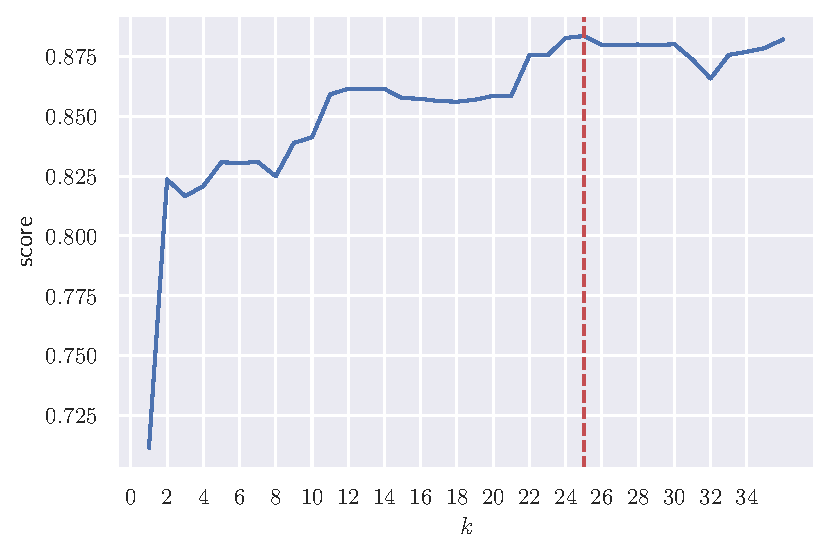
\includegraphics{kbest}
    \caption{Cross validation score for different $k$ values}%
    \label{fig:feature_cross}
\end{figure}

\begin{table}[H]
    \centering
    \caption{Selected features (25)}%
    \label{tab:features}
    \begin{tabular}{rlc}
\toprule
                   &  Variable &     Score \\
\midrule
1  &     \texttt{koi\_steff\_err1} &  0.193758 \\
2  &            \texttt{koi\_prad} &  0.184690 \\
3  &     \texttt{koi\_steff\_err2} &  0.170011 \\
4  &      \texttt{koi\_prad\_err1} &  0.164256 \\
5  &  \texttt{koi\_duration\_err2} &  0.156999 \\
6  &      \texttt{koi\_prad\_err2} &  0.154296 \\
7  &  \texttt{koi\_duration\_err1} &  0.153266 \\
8  &      \texttt{koi\_model\_snr} &  0.142149 \\
9  &      \texttt{koi\_srad\_err1} &  0.132922 \\
10 &   \texttt{koi\_time0bk\_err1} &  0.131132 \\
11 &          \texttt{koi\_period} &  0.128600 \\
12 &     \texttt{koi\_slogg\_err2} &  0.123361 \\
13 &   \texttt{koi\_time0bk\_err2} &  0.123268 \\
\bottomrule
\end{tabular}
\quad
\begin{tabular}{rlc}
\toprule
                   &  Variable &     Score \\
\midrule
14 &    \texttt{koi\_slogg\_err1} &  0.120881 \\
15 &          \texttt{koi\_steff} &  0.115671 \\
16 &   \texttt{koi\_period\_err2} &  0.109981 \\
17 &   \texttt{koi\_period\_err1} &  0.108709 \\
18 &    \texttt{koi\_insol\_err2} &  0.108357 \\
19 &          \texttt{koi\_depth} &  0.106608 \\
20 &    \texttt{koi\_insol\_err1} &  0.105152 \\
21 &           \texttt{koi\_srad} &  0.102525 \\
22 &          \texttt{koi\_insol} &  0.102372 \\
23 &            \texttt{koi\_teq} &  0.100868 \\
24 &         \texttt{koi\_impact} &  0.099700 \\
25 &                 \texttt{dec} &  0.099228 \\
\, & & \\
\bottomrule
\end{tabular}

\end{table}